\section{Theory and experimental setup}
\subsection{Metal-semiconductor junctions}
\hl{On peut utiliser MS pour dire metal-semiconductor junction}
\emph{What happens when we put a type n semiconductor in contact with a metal}
\begin{figure}[h]
    \centering
    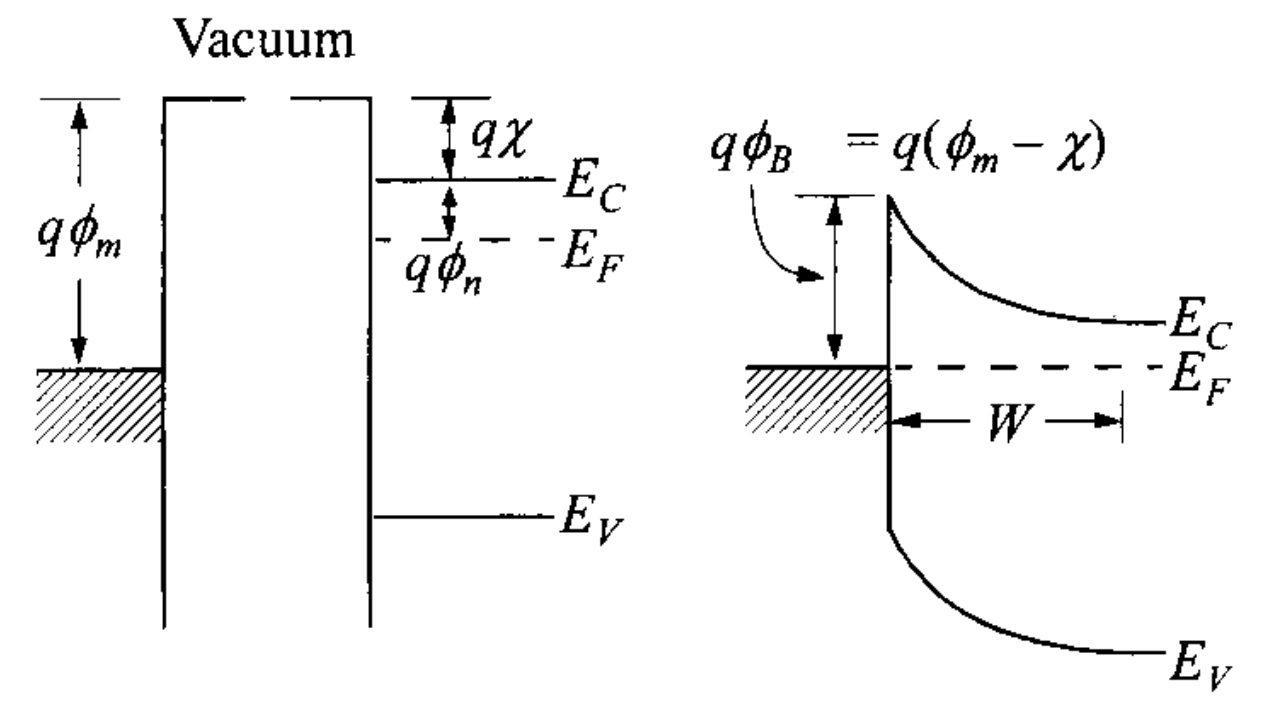
\includegraphics[width=12cm]{figures/schottky_barrier.png}
    \caption{}
    \label{fig:schottky_barrier}
\end{figure}
\begin{equation} \label{eq:barrier_height}
    \phi_b = \phi_m - \chi
\end{equation}
$q \phi_b$ is the barrier height of the metal-semiconductor contact.
It is this barrier that must be surmounted by electrons flowing from the metal into the semiconductor \cite{sze_physics_2007}.

We neglect surface-state effects (but \autoref{eq:barrier_height} is still generally valid \cite{sze_physics_2007}).
Even if contact is not perfect and a very
thin high barrier separating metal and semiconductor still remains as in l(c), this barrier is usually so thin ($\sim 10$ \AA) that electrons can easily pass through it by tunnelling \cite{rhoderick_physics_1970}


\subsection{Measurement of barrier height}
\hl{Alternativement une sous-section pour chaque méthode}
In this work the Schottky barrier of a Au-Si \hl{??} MS was determined using two different methods:
\begin{itemize}
    \item Current-Tension curves
    \item Photoelectric measurement
\end{itemize}


\paragraph{Current-Tension curves}
The principal mechanism responsible for the current flow at the majority of Schottky diodes on non-degenerate semiconductors has been shown by various studies to be the thermionic emission process \cite{tung_recent_2001}.
\begin{equation} \label{eq:IV-curve}
    V = \frac{n k_N T}{q} \ln \left( \frac{I}{I_S} +1 \right) + RI
\end{equation}


A $100 \%$ increase in $A^{**}$ will cause an increase of only $0.018$ V in $\phi_b$.


Even though $n$ is known as the  "ideality" factor, its numerical value actually reflects the departure from ideality; namely, the larger $n$ is, the less "ideal" is said of the SB \cite{tung_recent_2001}.
Generally speaking, the ideality factor is an indicator of the bias dependence of the SBH. With increasing forward bias, there is a tendency for the effective SBH which controls the current transport to also increase, giving rise to $n > 1$.

\paragraph{Illumination of the sample}


\subsection{Setup for I-V measures}
Sample was put in cryostat and studied for temperatures between $124 \pm ?$ and $296\pm?$ K, function generator sweeped tension between $0$ and $2.5$ V, measured current.

The curves were fit using \autoref{eq:IV-curve} to obtain parameters blablabla.
Then $\phi_b$.
